\chapter{Análisis de tecnologías a utilizar}
\label{cap:analisis_tecnologias}

\section{Análisis de las tecnologías Frontend}
\label{sec:frontend}
En la actualidad existen multitud de opciones en el mercado para el desarrollo de tecnologías móviles. A continuación se describen las tecnologías más populares y utilizadas en la actualidad para el desarrollo de aplicaciones móviles.

\subsection{Desarrollo nativo}
\label{subsec:nativo}
En primer lugar tenemos las tecnologías de \textbf{desarrollo nativo}, es decir, las tecnologías que permiten la creación de aplicaciones específicamente diseñadas
para un sistema operativo en concreto. Dichas tecnologías son: 

\begin{itemize}
    \item \href{https://kotlinlang.org/}{\textbf{Kotlin.}} Kotlin es un lenguaje que permite desarrollar aplicaciones para todas las plataforams soportadas por Android, siendo Android Studio
    el entorno de desarrollo integrado (IDE) principal para la creación de aplicaciones nativas en dicho sistema operativo. Una de las ventajas más destacas es su 
    total interoperabilidad con Java, lo que facilita el uso de bibliotecas escritas en Java dentro de proyectos desarrollados en Kotlin. Además, el lenguaje proporciona mecanismos
    avanzados de seguridad frente a valores nulos, lo que ayuda a prevenir errores durante la ejecución de las aplicaciones. Entre sus deventajas destaca que, aunque la popularidad ha crecido, aún no alcanzar
    el nivel de adopción de Java, lo que puede dificultar encontrar soluciones a problemas específicos. Asimismo, aunque existen iniciativas para su uso multiplataforma, Kotlin sigue estando principal,emte 
    orientado al desarrollo de aplicaciones en Android.

    \begin{figure}[h] 
        \centering
        
\includegraphics[width=0.4\textwidth]{../capitulos/img/Kotlin_logo.svg.png} 
        \caption{Logo de Kotlin}
        \label{fig:logo_kotlin}
    \end{figure}
    

    \item \href{https://www.swift.org/}{\textbf{Swift.}} Es un lenguaje, diseñado específicamente para crear aplicaciones de alto rendimiento y con una sintaxis clara y moderna. En este caso el IDE es XCode utilizado para el desarrollo nativo en las plataformas de Aplle, como iOS y macOS. 
    Swift se caracteriza por su seguridad, facilidad de uso y capacidades de optimización, lo que lo convierte en una buena opción para el desarrolo de aplicaciones en el ecosistema de Apple. Como principales carácteristicas de Swift podemos destacar una \textbf{sintaxis simple y moderna}, 
    un \textbf{alto rendimiento} debido a su compilador avanzado permite ejecutar aplicaciones de manera eficiente, \textbf{seguridad} gracias a su sistema de tipos fuertes y a la prevención de errores en tiempo de ejecución, e \textbf{interoperabilidad con Objetive-C} lo que facilita la integración de código. 
    Sin embargo, una de las principales deventajas de Swift es similar a la mencionada anteriormente en Kotlin, \textbf{la duplicidad de esfuerzos} en el desarrollo de aplicaciones multiplataforma. Las aplicaciones desarrolladas con Swift
    obligan a los desarrolladors a crear aplicaciones independientes para otras plataformas. 
    
    \begin{figure}[h] 
        \centering
        
\includegraphics[width=0.3\textwidth]{../capitulos/img/images.png} 
        \caption{Logo de Swift}
        \label{fig:logo_swift}
    \end{figure}

\end{itemize}

\subsection{Desarrollo Híbrido}
\label{subsec:hibrido}
Las tecnologías de desarrollo híbrido representan una alternativa eficaz en el ámbito de aplicaciones multiplataforma. Estas tecnologías permiten crear una única 
base de código que puede ser ejecutada tanto en dispositivos con sistema operativo iOS como en Android. La principal ventaja de este enfoque es la optimización de los recursos,
tanto económicos como operativos, ya que reduce significativamente los costes asociados al desarrallo y mantenimiento de las aplicaciones. Al utilizar un solo lenguaje y una 
única estructura de programación, se consigue implementar una solución funcional para ambas plataformas. Además, permite una mejor experiencia al usuario, garantizando que la aplicación
tenga un comportamiento y apariencia similares. Algunos ejemplos de esta tecnología son:

\begin{itemize}
    \item \href{https://ionicframework.com/}{\textbf{Ionic.}} Es un framework de código abierto que permite crear aplicaciones móviles, web y de escritorio utilizando tecnologías webs, como HTML, CSS y JavaScript.
    Se integra con diferentes frameworks frontend como Angular React o Vue, lo que permite a los desarrolladores utilizar el conjunto de herramientas y librerías de su preferencia. Además, Ionic 
    tiene componentes nativos que proporcionan una biblioteca de elementos visuales optimizados para dispositivos móviles. Cuenta también con una \textbf{amplia comunidad} y herramientas adicionales para la integración 
    con servicios de backend y otras tecnologías.

    \begin{figure}[h] 
        \centering
        
\includegraphics[width=0.4\textwidth]{../capitulos/img/ionic-itop.png} 
        \caption{Logo de Ionic}
        \label{fig:logo_ionic}
    \end{figure}

    \item \href{https://flutter.dev/}{\textbf{Flutter.}} Flutter es un framework de código abierto desarrollado por Google que permite crear aplicaciones nativas multiplatadorma con una única base de código. Utiliza el lengujae de programación Darrt
    y proporciona un enfoque único para desarrollar aplicaciones móviles, web y de escritorio. Tiene un \textbf{alto rendimiento} debido a que utiliza un motor gráfico y compila directamente a código nativo, lo que garantizando
    un rendimiento similar al de aplicaciones nativas. Además. cuenta con \textit{Hot Reload} que facilita el desarrollo rápido al permitir que lo cambios en el código se reflejen instantáneamente en la aplicación
    sin tener que recompilar por completo.

    \begin{figure}[h] 
        \centering
        
\includegraphics[width=0.4\textwidth]{../capitulos/img/flutter.png} 
        \caption{Logo de Flutter}
        \label{fig:logo_flutter}
    \end{figure}

    \item \href{https://reactnative.dev/}{\textbf{React Native.}} React Native es un framework de código abierto desarrollado por Facebook que permite crear aplicaciones móviles nativas utilizando JavaScript y React. A diferencia de otros frameworks
    híbridos, React Native no se limita a emular una experiencia nativa, en su lugar, \textbf{genera componentes nativos}, lo que permite un rendimiento más cercano al de una aplicación pura. Además cuenta con una 
    \textbf{amplia comunidad} y una gran cantidad de librerías y herramientas que facilitan el desarrollo de aplicaciones.
    \begin{figure}[h] 
        \centering
        
\includegraphics[width=0.5\textwidth]{../capitulos/img/react.png} 
        \caption{Logo de React Native}
        \label{fig:logo_react}
    \end{figure}
    \item \href{https://dotnet.microsoft.com/apps/xamarin}{\textbf{Xamarin.}} Es un framework de código abierto desarrollado por Microsoft que permite crear aplicaciones móviles nativas para iOS y Android utilizando C\# y .NET. Xamarin permite compartir hasta un 90\% del código.
    Además, proporciona acceso a las API nativas de cada plataforma, lo que permite a los desarrolladores crear aplicaciones con una \textbf{experiencia de usuario nativa}. También se integra a la perfección con herramientas del ecosistema de Microsoft, como Visual Studio, facilitando
    el desarrollo y la depuración de aplicaciones.
    \begin{figure}[h] 
        \centering
        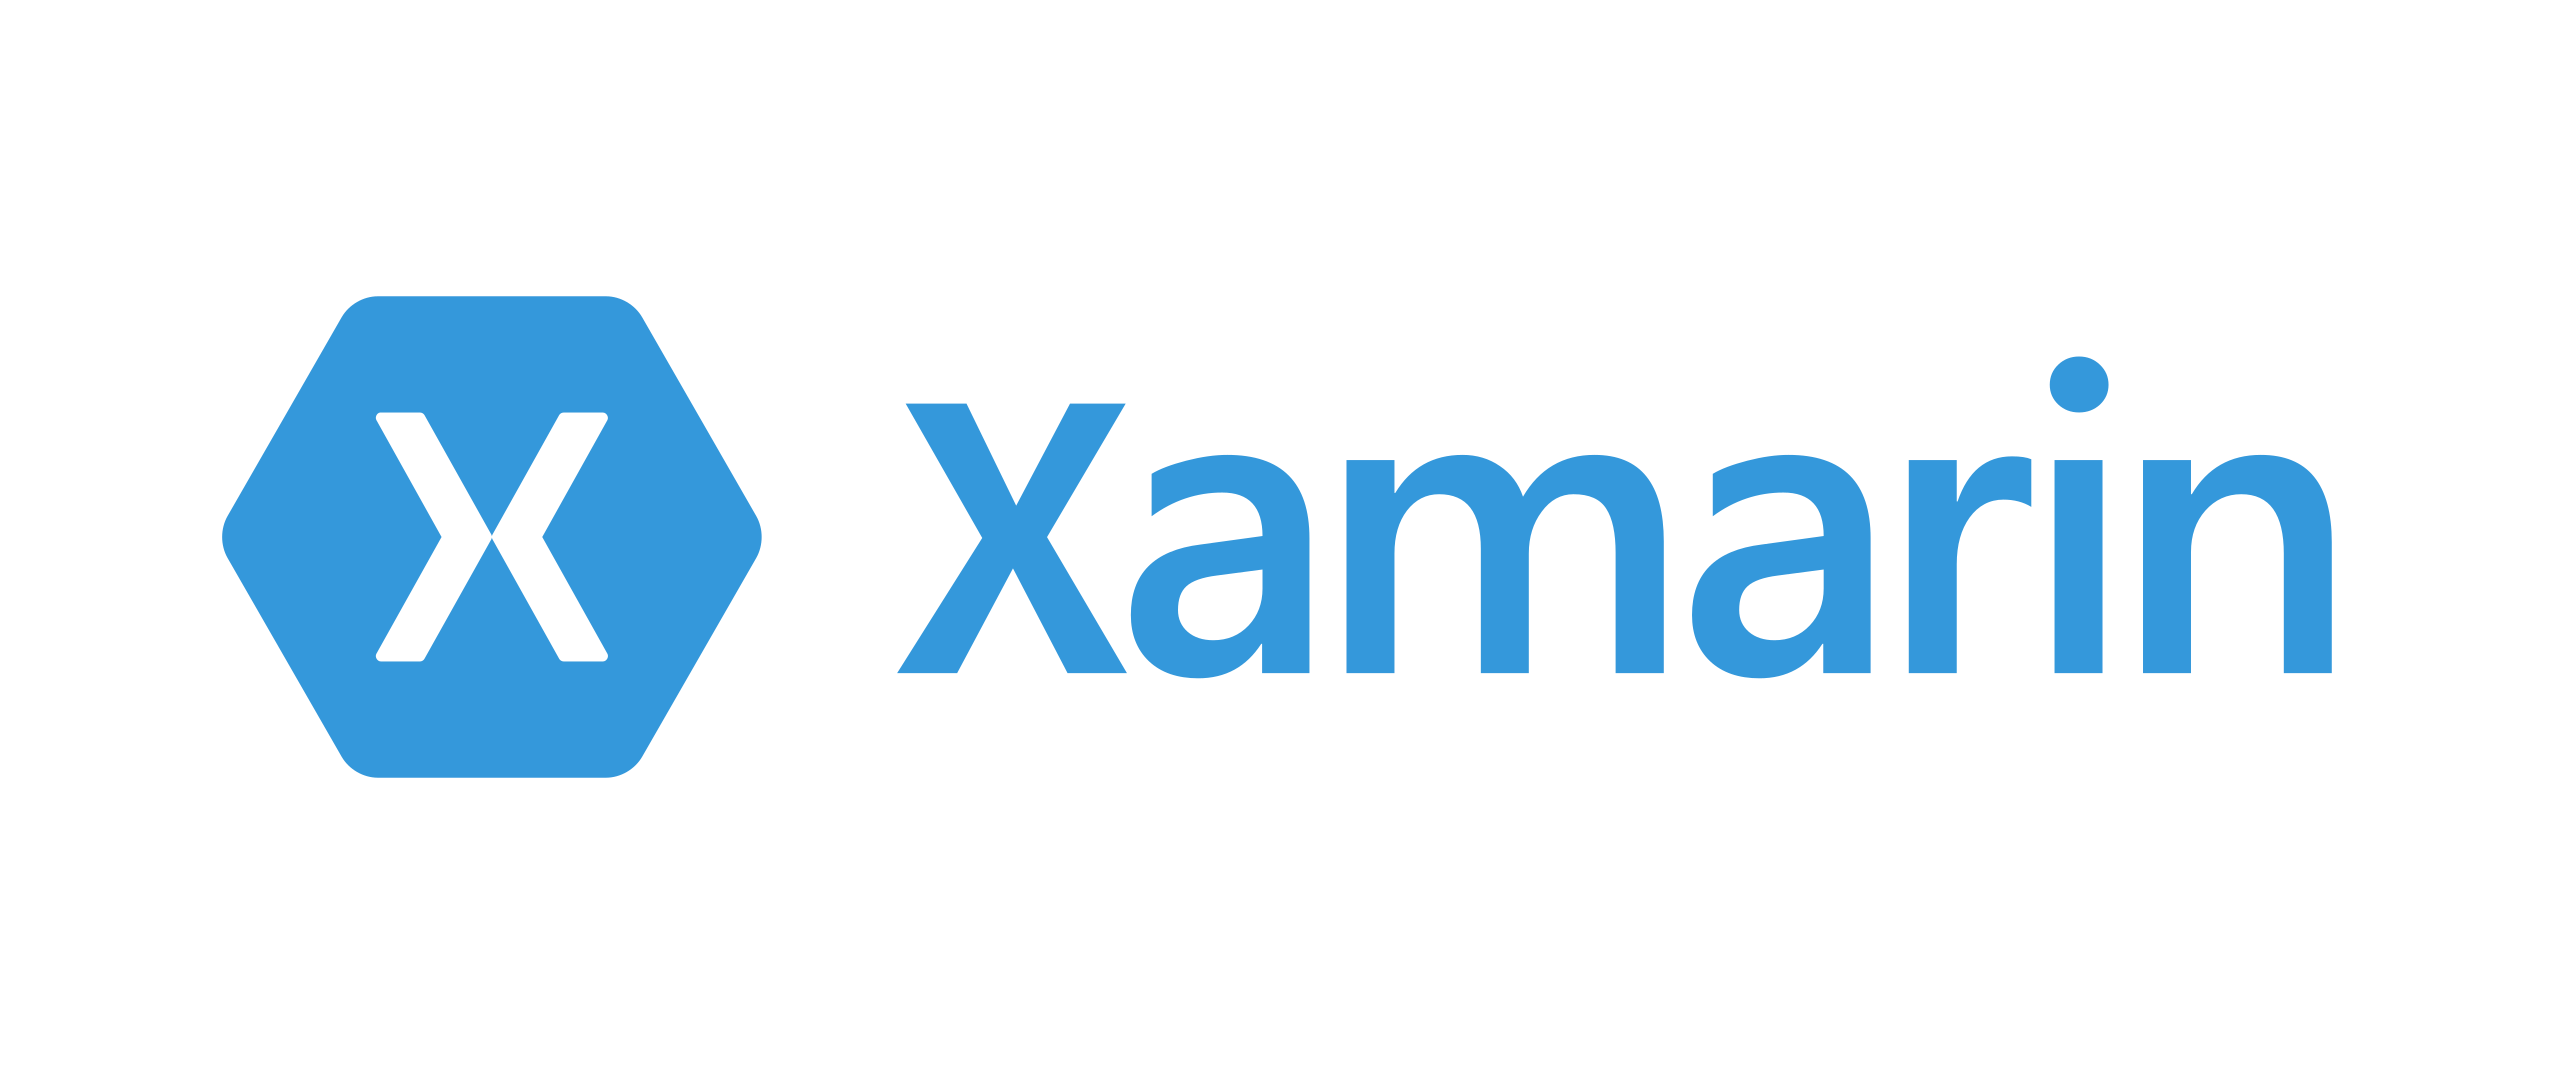
\includegraphics[width=0.5\textwidth]{../capitulos/img/xamarin.png} 
        \caption{Logo de Xamarin}
        \label{fig:logo_xamarin}
    \end{figure}

\end{itemize}



\subsection{Tabla comparativa de tecnologías front-end}
\label{subsec:comparativa}
La siguiente tabla ofrece una comparación entre las tecnologías más populares en el desarrollo frontend de aplicaciones móviles, 
evaluando aspectos clave como el lenguaje de programación, rendimiento, disponibilidad de componentes de UI, tamaño de la comunidad, soporte de funcionalidad \textit{Hot Reload} e 
integración con otros sistemas y herramientas. Esta información proporciona una visión global de las fortalezas y limitaciones de cada opción, facilitando así la selección de la tecnología que mejor se ajuste a los requisitos específicos del proyecto.
\begin{table}[ht]
    \centering
    \scalebox{0.7}{
    \begin{tabular}{|c|c|c|c|c|c|c|}
        \hline
        \textbf{} & \textbf{Lenguaje} & \textbf{Rendimiento} & \textbf{Componentes UI} & \textbf{Comunidad} & \textbf{Hot Reload} & \textbf{Integración} \\
        \hline
         \textbf{Kotlin} & Java & Nativo & Componentes Nativos & Grande & No  & Herramientas Nativas \\
        \hline
        \textbf{Swift} & Swift & Nativo & Componentes Nativos & Grande & No & Herramientas Nativas \\
        \hline
        \textbf{Ionic} & JavaScript & Buen Rendimiento & Componentes Nativos & Grande & Sí & Buen Soporte \\
        \hline
        \textbf{Flutter} & Dart & Cercano a Nativo & Personalizados & Activa & Sí & Buen Soporte \\
        \hline
        \textbf{React Native} & JavaScript & Buen Rendimiento & Componentes Nativos & Grande & Sí & Buen Soporte \\
        \hline
        \textbf{Xamarin} & C\# & Buen Rendimiento & Componentes Nativos & Grande & Sí & Integración Microsoft \\
        \hline
    \end{tabular}
    }
    \caption{Tabla comparativa de tecnologías front-end}
    \label{tab:comparativa}
\end{table}

En conclusión, la tabla destaca cómo cada tecnología ofrece un conjunto único de beneficios. Las opciones nativas como Kotlin y Swift son preferibles para aplicaciones que requieran un rendimiento óptimo y un uso extensivo de componentes específicos de la plataforma. 
Sin embargo, soluciones como Flutter y React Native se presentan como alternativas atractivas para el desarrollo multiplataforma debido a su rendimiento cercano al nativo, su comunidad activa y sus herramientas avanzadas de desarrollo rápido como \textit{Hot Reload}. 


\newpage

\section{Analisis de las tecnologías Backend}
\label{sec:backend}
Otra de las decisiones que hay que tomar es la tecnología back-end que permita la comunicación entre la aplicación y la base de datos. A continuación vamos a ver las diferentes tecnologías que hay para ello:

\subsection{Firebase}
\label{subsec:firebase}
\href{https://firebase.google.com/}{Firebase} es una plataforma de Google que ofrece una amplia variedad de servicios backend, lo que incluye \textbf{bases de datos en tiempo real}
como FireStore y Realtime Database. Además. proporciona servicios de autenticación, almacenamiento de archivos, notificaciones push, análisi y más.
No requiere gestión de servidores debido a que es completamente serverless. Cuenta con una \textbf{fácil integración} con Flutter debido a que 
tiene SDks nativos para dicha tecnología, lo que simplifica mucho el desarrollo en comparación con otras tecnologías que requieren la integración manual. Sin embargo, 
Firebase tiene un \textbf{coste} asociado al uso de sus servicios, lo que puede ser un inconveniente para proyectos con presupuestos limitados. También tiene una \textbf{dependencia de Google}, porque todo esta alojados
en la infraestructura de Google, lo que puede generar dependecia a largo plazo.
\begin{figure}[h] 
    \centering
    
\includegraphics[width=0.5\textwidth]{../capitulos/img/Firebase.png} 
    \caption{Logo de Firebase}
    \label{fig:logo_firebase}
\end{figure}

\subsection{Node.js con Express}
\label{subsec:node}
\href{https://nodejs.org/}{Node.js} es un entorno de ejecución de JavaScript que permite ejecutar código JavaScript en el backend. Express es un 
framework ligero que permite construir aplicaciones web y APIs REST de manera rápida y sencilla. Además, es bastante útil para aplicaciones que manejan 
un alto número de solicitudes simultáneas. Para el almacenamiento de datos se pueden usar bases de datos realacionales como \textbf{MySQL} o \textbf{PostgreSQL} o bases de datos NoSQL como \textbf{MongoDB}.
Gracias a npm (\textit{Node Package Manager}), hay miles de paquetes disponibles que permiten acelerar el proceso de desarrollo. También es una tecnología \textbf{flexible}, porque permite elegir el tipo de base de datos.
Por el contrario tiene una \textbf{Complejidad de gestión del servidor}. Aunque Express es minimalista, la creación y gestión de servidores, puede ser más compleja en comparación con soluciones serverless. Además, la \textbf{curva de aprendizaje} puede ser más pronunciada para desarrolladores que no tienen experiencia previa con JavaScript.

\begin{figure}[h] 
    \centering
    
\includegraphics[width=0.3\textwidth]{../capitulos/img/Node.js.png} 
    \caption{Logo de Node.js}
    \label{fig:logo_node}
\end{figure}

\subsection{Django}
\label{subsec:django}
Es un framework web de alto nivel escrito en Python que facilita la creación de aplicaciones webs seguras y escalables. Junto con \textbf{Django REST Framework}, permite exponer APis REST de forma 
rápida y eficiente. Se integra bien con bases de datos relacionales como \textbf{PostgreSQL} y \textbf{MySQL}. \href{https://www.djangoproject.com/}{Django} proporciona un \textbf{rápido desarrollo} debido a que incluye una gran cantidad de herramientas listas para usar (\textit{autenticación, administración, etc.}).
Además, tiene carácteristicas de seguridad incorporadas, como protección CSRF, gestión de contraseñas seguras y más. También proporciona \textbf{gestión automática de bases de datos} sin tener que escribir consultas SQL Manuales. 
Sin embargo, Django puede ser algo pesado para proyectos más pequeños o simples. Además, la \textbf{curva de aprendizaje} puede ser pronunciada para desarrolladores que no tienen experiencia previa con Python.

\begin{figure}[h] 
    \centering
    
\includegraphics[width=0.4\textwidth]{../capitulos/img/django.png} 
    \caption{Logo de Django}
    \label{fig:logo_django}
\end{figure}

\subsection{Ruby on Rails}
\label{subsec:rails}
\href{https://rubyonrails.org/}{Ruby} on Rails es un framework MVC (\textit{Modelo-Vista-Controlador}) escrito en Ruby, que permite desarrollar aplicaciones web y APis de manera rápida. Rails se integra
perfectamente con bases de datos relacionales como \textbf{PostgreSQL} o \textbf{MySQL}. Una facilidad que incorpora Ruby on Rails es la \textbf{Convención sobre configuración}, 
lo que significa que muchas decisiones están predefinidas para que el desarrollador no tenga que configurarlas manualmente, acelerando el proceso de desarrollo.
También \textbf{facilita la interacción} con la base de datos relacionales. Sin embargo, Aunque Rails es excelente para aplicaciones web, no es tan común en el desarrollo de APIs para 
aplicaciones móviles.

\begin{figure}[h] 
    \centering
    
\includegraphics[width=0.4\textwidth]{../capitulos/img/ruby.png} 
    \caption{Logo de Ruby on Rails}
    \label{fig:logo_ruby}
\end{figure}


\subsection{Tabla comparativa de tecnologías back-end}
\label{subsec:comparativa2}
La tabla siguiente compara algunas de las tecnologías back-end más comunes en el desarrollo de aplicaciones web y móviles, 
evaluando aspectos como el lenguaje de programación, las bases de datos soportadas, la gestión del estado, la integración con APIs y la popularidad general. 
\begin{table}[H]
    \centering
    \resizebox{1.3\textwidth}{!}{
    \begin{tabular}{|c|c|c|c|c|c|}
        \hline
        \textbf{} & \textbf{Lenguaje} & \textbf{BD Soportada} & \textbf{Gestión del estado} & \textbf{Integración con API} & \textbf{Popularidad} \\
        \hline
        \textbf{Firebase} & - & Firebase, Realtime DB & Serverless, en tiempo real & APIs nativas de Firebase & Muy alta \\
        \hline
        \textbf{Node.js} & JavaScript & MongoDB, MySQL, PostgreSQL & Depende de la implementación & Muy flexible & Muy alta \\
        \hline
        \textbf{Django} & Python & PostgreSQL, MySQL & ORM Propio & Django REST Framework & Alta \\
        \hline
        \textbf{Ruby on Rails} & Ruby & PostgreSQL, MySQL & ActiveRecord ORM & RESTful API fácil de implementar & Media \\
        \hline
    \end{tabular}
    }
    \caption{Tabla comparativa de tecnologías back-end}
    \label{tab:comparativa2}
\end{table}

En conclusión, esta tabla muestra cómo cada tecnología back-end aporta ventajas específicas. Firebase destaca en aplicaciones en tiempo real y serverless, ideal para proyectos rápidos 
que requieren menos mantenimiento de servidores. Node.js es muy flexible y compatible con diferentes bases de datos, adaptándose bien a aplicaciones escalables. Django y Ruby on Rails ofrecen 
una estructura robusta y sencilla de implementar, siendo opciones populares para aplicaciones que necesitan un backend consolidado.

\newpage


\section{Justificación de la elección de tecnologías}
\label{sec:justificacion}
Tras analizar las diferentes tecnologías disponibles para el desarrollo de la aplicación, he decidido utilizar \textbf{Flutter} como tecnología front-end 
porque presenta varias ventajas significativas frente al resto de alternativas. Una de las razones más destacadas es su capacidad de desarrollo multiplataforma, 
que permite crear una única base de código que se ejecuta tanto en Android, como en iOS, web y aplicaciones de escritorio, lo que ahorra tiempo 
y esfuerzo en comparación con desarrollar código nativo para cada plataforma por separado. Además, Flutter ofrece un rendimiento cercano al 
de las aplicaciones nativas, gracias a su motor gráfico Dart, que se compila en código nativo. Otra ventaja es el sistema de Hot Reload, que permite 
a los desarrolladores visualizar los cambios en tiempo real, sin tener que recompilar por completo. Tiene también una enorme capacidad de 
personalización, simplificando la tarea. Además, al estar respaldado por Google,, recibe soporte continuo.



En cuanto a la tecnología back-end, he decidido utilizar \textbf{Firebase} porque ofrece una serie de ventajas que lo hacen destacar frente a las
otras alternativas. Para empezar, Firebase proporciona un backend completo, lo que significa que no es necesario gestionar servidores ni 
preocuparse por la configuración y el mantenimiento. La integración de la autenticación de usuarios es también uno de sus puntos fuertes, ya que 
Firebase Auth facilita la implementación de los mismos. Otra razón para elegir Firebase es su base de datos en tiempo real, que permite 
sicronización instantánea de datos. Además, tiene una gran integración con servicios de Google, optimizando la monitorización del rendimiento.

\newpage